%\textsf{Web of Things architecture \cite{Wot2017arch}, Thing Description \cite{Wot2017td} and
%scripting API \cite{Wot2017script}.}

The WoT architecture\cite{Wot2017arch} defines three basic entities that can be organized in a various set of configurations and topologies based on a concrete deployment scenario:

\begin{itemize}
	\item A \textbf{WoT Thing} represents a physical or virtual IoT device and exposes a network-facing API for interaction.
	Each WoT Thing has an associated Thing Description (TD)\cite{Wot2017td} that is a set of metadata describing relevant information about the Thing, such as general information, available interactions, communication and security mechanisms.
	A typical example of a WoT Thing might be a garage door controller, providing a number of actions that can be performed on a garage door, i.e. \textit{open}, \textit{close}, etc.
	\item A \textbf{WoT Client} is an entity that wants to perform an action on a WoT Thing.
	It is able to consume a TD provided by a WoT Thing and issue actions on exposed WoT interfaces.
	For example a WoT Client might be a browser or an application on a user's smartphone that allows user to operate the garage door controller. 
	\item A \textbf{WoT Servient} can be viewed as a combination of above two, i.e. an entity that is both providing one or more WoT things and also at the same time is able to operate as WoT Client on other WoT things.
	An example of a WoT servient is a home gateway device that acts as a WoT client towards home appliance WoT things (such as different lights and sensors) and also exposes some higher level virtual devices (such as all the lights in the living room) in form of the WoT Things available for user's smartphone WoT Client.
\end{itemize}

Internally a typical architecture of a WoT Servient is shown in Figure~\ref{fig-fservient}. 
In addition to a Thing Description (TD) it also has WoT Binding Templates that can be used to instantiate a TD for a particular IoT protocol binding, such as OCF, COAP etc. 
The last remaining part is WoT Scripting API, which is an optional component that allows implementing the Thing logic in a higher-level programming language and browser-like environment (such as JavaScript). 

\begin{figure}[!t]
\centering
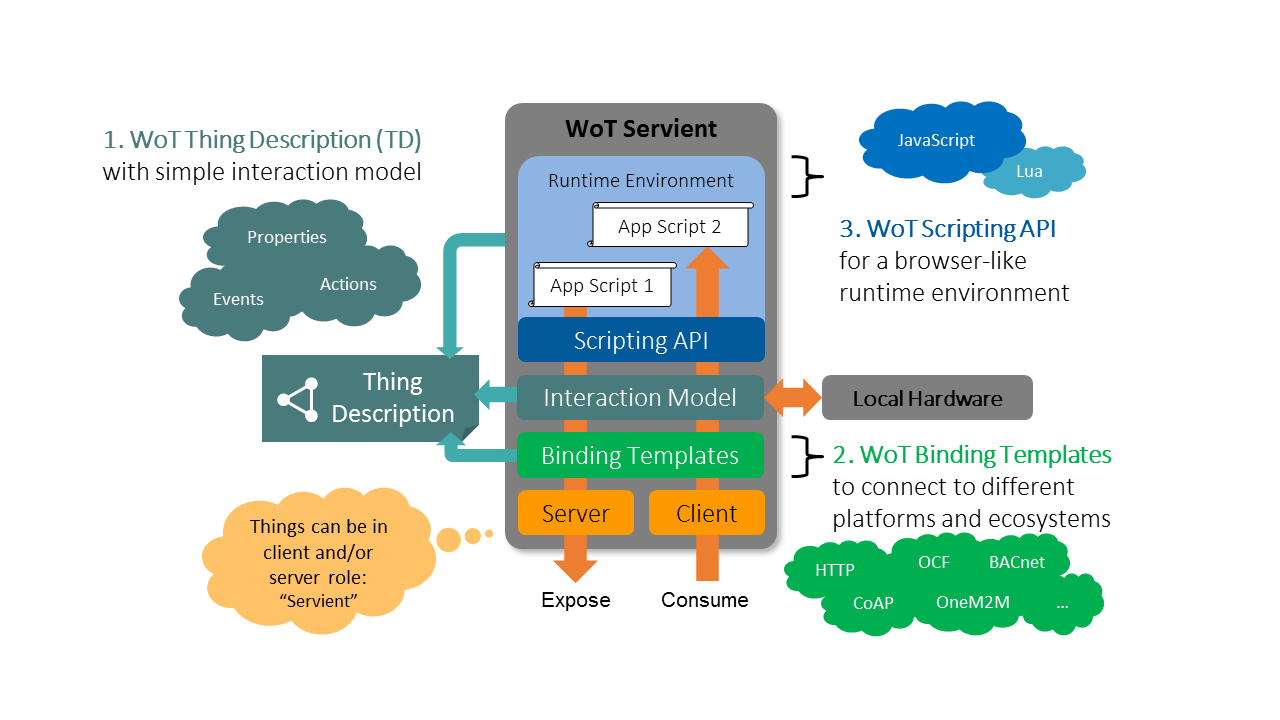
\includegraphics[width=4in]{figures/wot-servient.png}
\caption{WoT Servient architecture}
\label{fig-fservient}
\end{figure}


